% ----------------------------------------------------------------------
%  Pracovní úkoly
% ----------------------------------------------------------------------
\section{Pracovní úkoly}

\begin{enumerate}
\item Studium lomových ploch pomocí SEM.

\item Měření střední velikosti zrna polykrystalického vzorku. K vyhodnocení snímku ze scanovacího elektronového mikroskopu použijte kruhovou metodu.

\item Určení frakčního objemu dané fáze ve vícefázovém materiálu. Použijte specializované programové vybavení pro obrazovou analýzu.
\end{enumerate}

% ----------------------------------------------------------------------
%  Teoretická část
% ----------------------------------------------------------------------
\section{Teoretická část}

Skenovací elektronová mikroskopie (SEM) je zobrazovací metoda, která využívá ostře fokusovaný svazek elektronů namísto světelné optiky. Primární elektrony (PE) emitované katodou jsou urychlovány kladným napětím na anodě a elektromagnetickými čočkami zaostřeny na povrch vzorku. Vychylovací cívky umožňují, aby svazek postupně přejížděl po vymezené ploše bod po bodu a řádek po řádku, podobně jako v televizní technice. Signál z detektoru je synchronizován s pohybem svazku a jeho intenzita moduluje jas obrazu.

Po dopadu na povrch vzorku pronikají elektrony do určité hloubky, kde dochází k pružnému i nepružnému rozptylu. Při nepružném rozptylu předávají energii elektronům pevné látky a krystalové mřížce, což vede ke vzniku sekundárních elektronů (SE), Augerových elektronů, charakteristického rentgenového záření a dalších signálů. Pro běžné účely se využívají zejména:
\begin{itemize}
    \item \textbf{Sekundární elektrony (SE)} – emitované z povrchu vzorku s energií menší než 50~eV, jejich intenzita závisí na topografii povrchu.
    \item \textbf{Zpětně odražené elektrony (BSE)} – jejich intenzita závisí na chemickém složení a krystalografické orientaci.
\end{itemize}

SEM umožňuje získat informace nejen o povrchové topografii, ale také o lokálních změnách chemického složení a některých fyzikálních vlastnostech vzorku. V této úloze se metoda SEM využívá pro:
\begin{enumerate}
    \item Studium lomových ploch intermetalické slitiny Fe$_3$Al při různých teplotách, kde se sleduje rozdíl mezi křehkým lomem při pokojové teplotě a tvárným lomem při 700~°C.
    \item Měření střední velikosti zrna polykrystalického vzorku pomocí kruhové metody, která vychází ze vztahu:
\begin{equation}
    d = \frac{3D}{2n\pi}
\end{equation}
    kde $D$ je průměr kružnice a $n$ počet protínajících zrn.
    \item Stanovení frakčního objemu fáze ve vícefázovém materiálu na základě kontrastu v BSE obraze, který závisí na průměrném atomovém čísle.
\end{enumerate}

Kontrast v BSE režimu je silnější v oblastech s vyšším průměrným atomovým číslem, což umožňuje rozlišit jednotlivé fáze. Pro přesné vyhodnocení se využívá obrazová analýza, zahrnující binarizaci snímku a výpočet podílu plochy dané fáze.

Celkovou chybu jsme spočetli podle vzorce

\begin{equation}
    \sigma = \sqrt{\sigma^2_{stat}+\sigma^2_{system}}
\end{equation}
\newpage
% ----------------------------------------------------------------------
%  Výsledky a zpracování měření
% ----------------------------------------------------------------------
\section{Výsledky a zpracování měření}

\subsection{Studium lomových ploch}

Studovali jsme intermetalickou slitinu na bázi $Fe_3Al$ v závislosti na teplotě podle \cite{bib:zadani}. Zajímala nás morfologie povrchu, proto jsme zvolili měření sekundárních elektronů. Závislost na teplotě jsme získali proměřením dvou vzorků, jeden tažený při pokojové teplotě, druhý při teplotě 700 °C. Na obrázku \ref{fig:lom_rt_combined} (vlevo) je snímek z elektronového mikroskopu vzorku taženého při pokojové teplotě, na obrázku \ref{fig:lom_rt_combined} (vpravo) je detailní snímek ve větším zvětšení. 

\begin{figure}[!h]
    \centering
    \begin{minipage}[b]{0.48\linewidth}
        \centering
        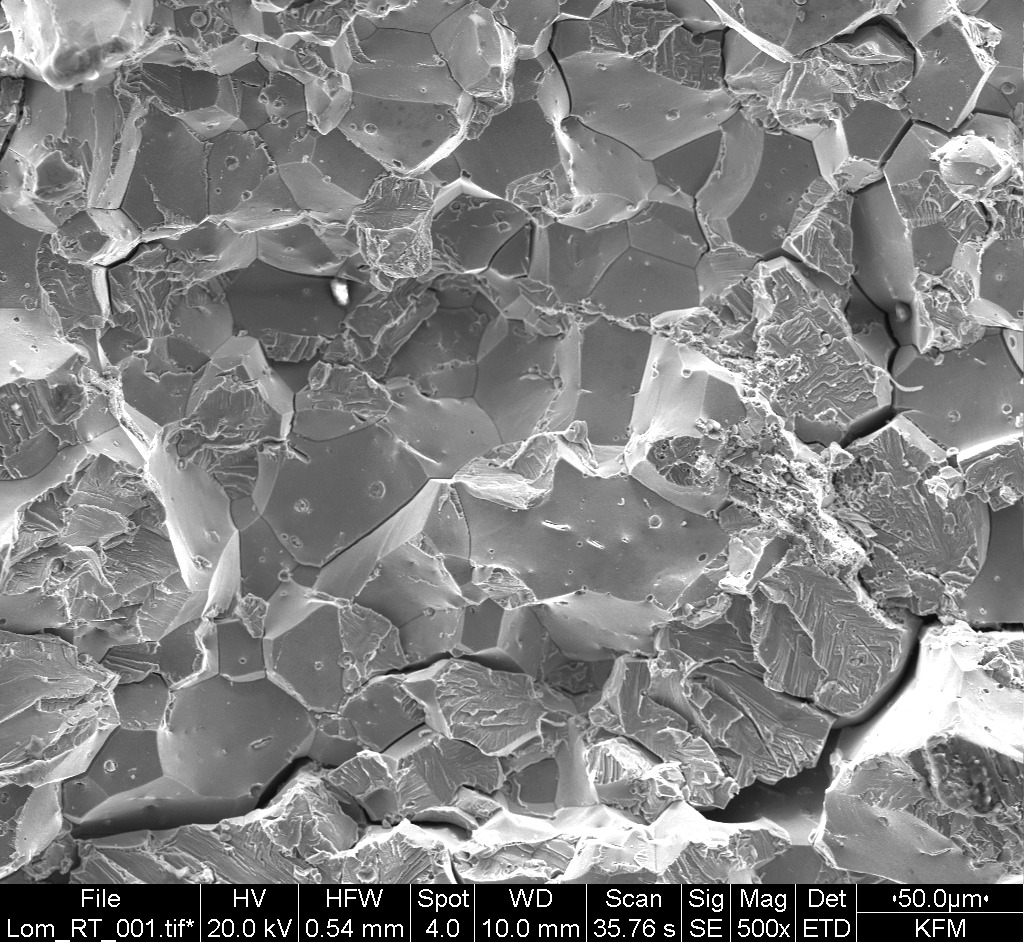
\includegraphics[width=\linewidth]{A18 - SEM/Lom_RT_001.jpg}
    \end{minipage}
    \hfill
    \begin{minipage}[b]{0.48\linewidth}
        \centering
        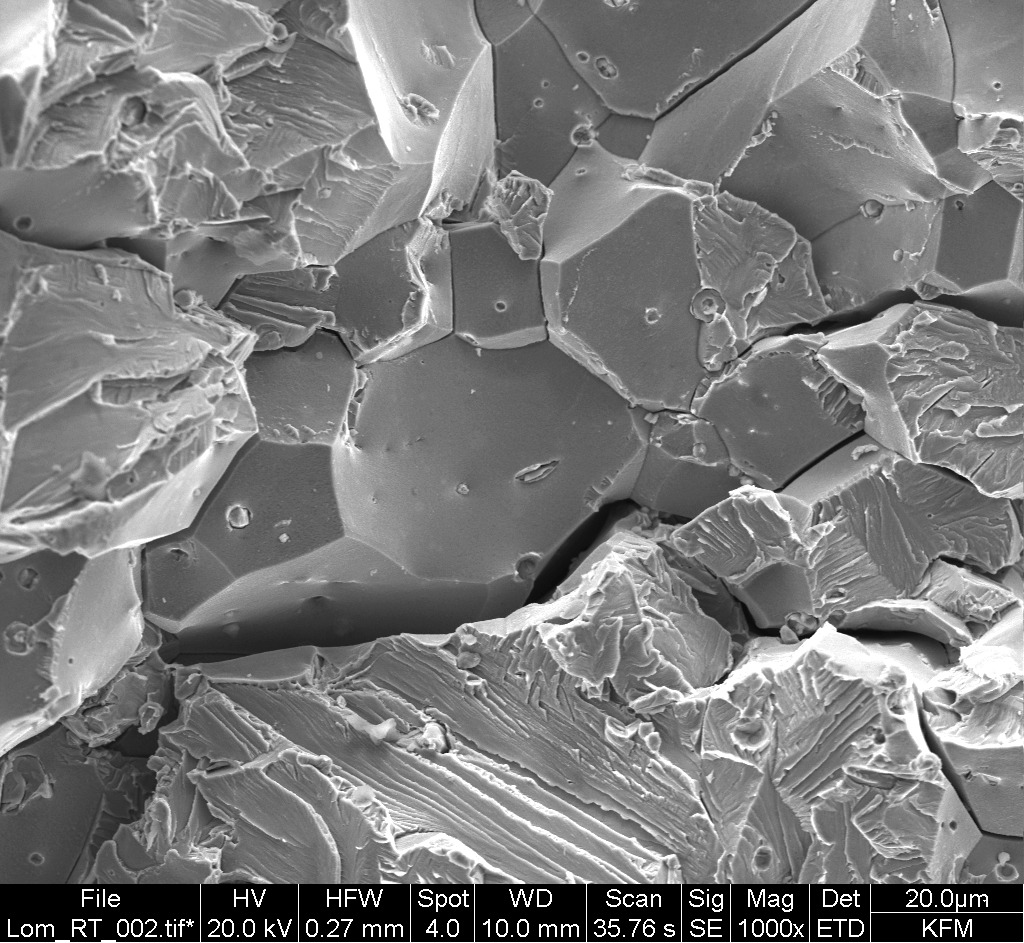
\includegraphics[width=\linewidth]{A18 - SEM/Lom_RT_002.jpg} % uprav dle potřeby
    \end{minipage}
    \caption{Snímky vzorku taženého při pokojové teplotě – vpravo s větším zvětšením}
    \label{fig:lom_rt_combined}
\end{figure}

Zvětšení uvedené v legendě pod obrázkem ztrácí význam, protože se jedná o poměř mezi šířkou velikosti okna v měřícím programu a šířkou měření vzorku. Legendu jsme však zanechali pro zachování ostatních parametrů. Vidíme, že se jedná o křehký lom. Lomová plocha se nachází mezi jednotlivými zrny, které jsme schopni na snímku odlišit. Tento lom se nazývá interkrystalický. V některých částech nedochází k oddělení sousedních zrn, ale k přelomení zrn dané geometrií zrn, kde je přelomení zrna přirozenější než jejich oddělování. Takovýto děj označujeme jako transkrystalický lom. Pokud bychom se podívali na opačnou stranu původního materiálu (před přetržením), viděli bychom negativ zobrazeného snímku. Obě části by do sebe zapadly.

Podobně na snímku \ref{fig:lom_700_combined} pozorujeme vzorek tažený při teplotě 700 °C.

\begin{figure}[!h]
    \centering
    \begin{minipage}[b]{0.48\linewidth}
        \centering
        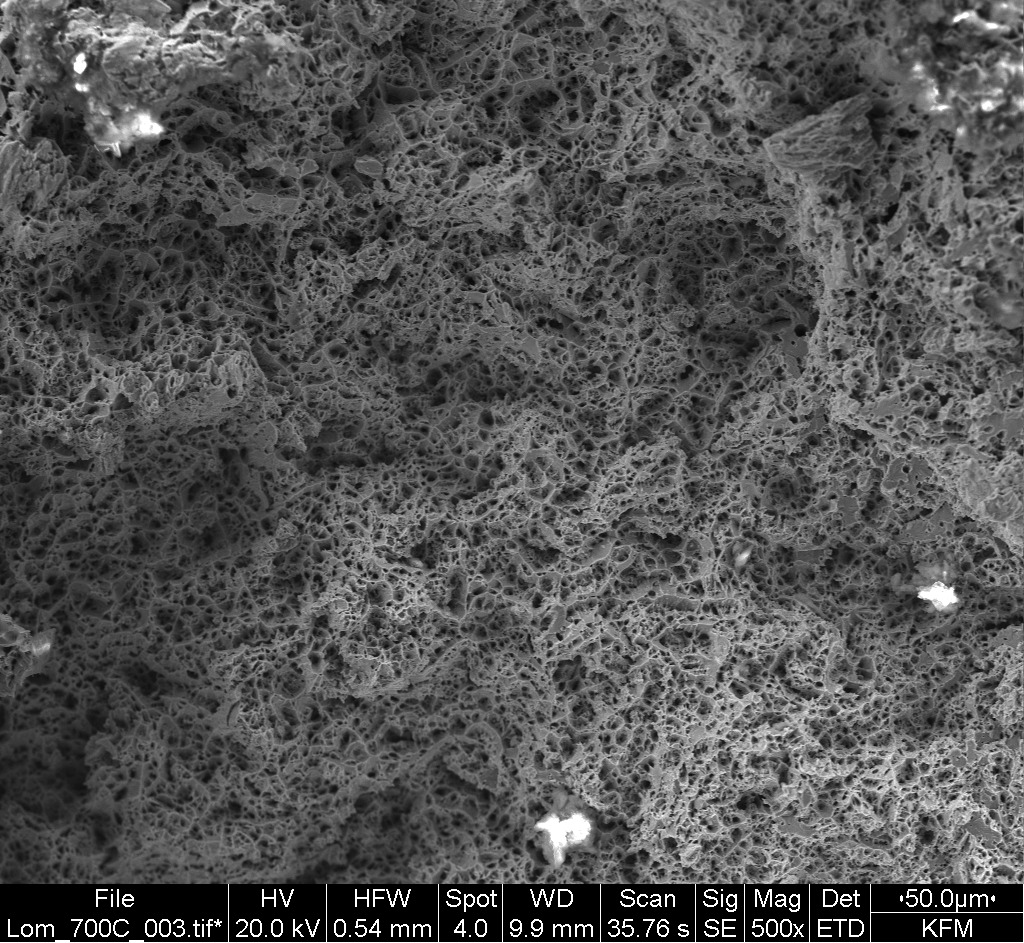
\includegraphics[width=\linewidth]{A18 - SEM/Lom_700C_003.jpg}
    \end{minipage}
    \hfill
    \begin{minipage}[b]{0.48\linewidth}
        \centering
        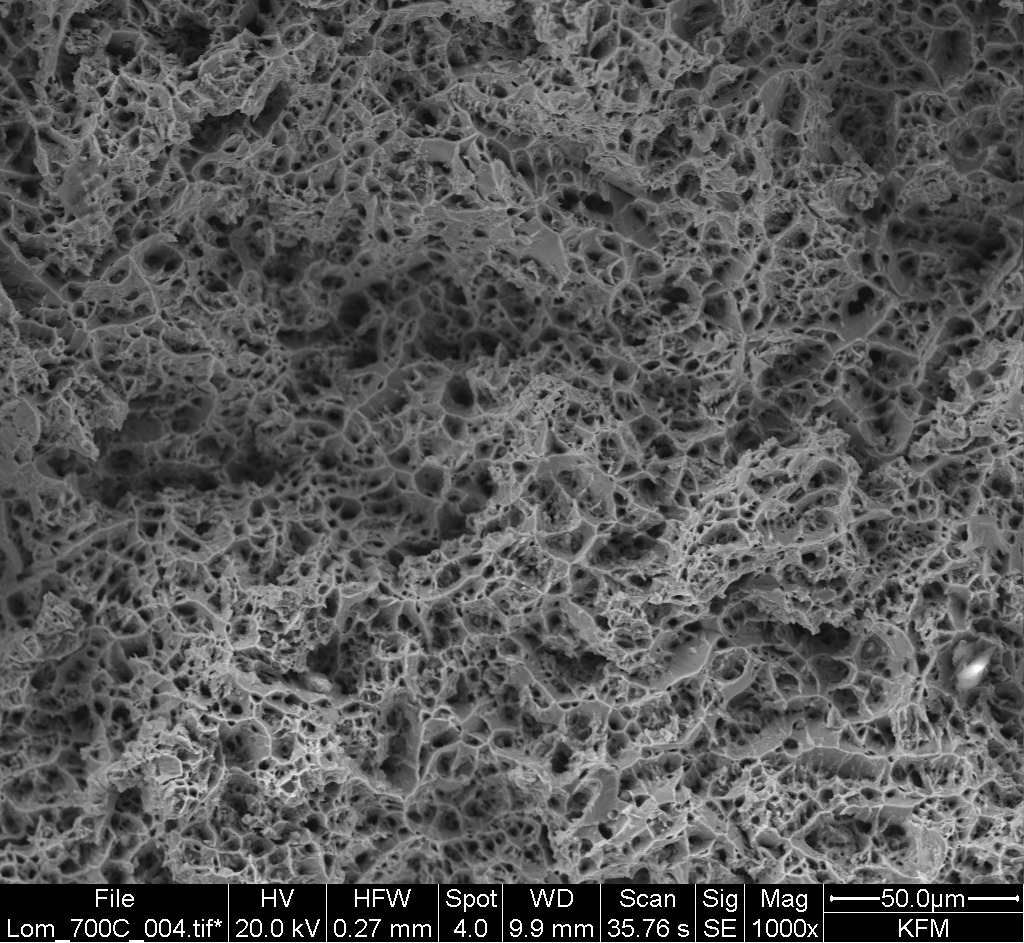
\includegraphics[width=\linewidth]{A18 - SEM/Lom_700C_004.jpg} % uprav dle potřeby
    \end{minipage}
    \caption{Snímky vzorku taženého při pokojové teplotě – vpravo s větším zvětšením}
    \label{fig:lom_700_combined}
\end{figure}

V tomto případě, na rozdíl od předchozího vzorku, pozorujeme tzv. tvárný důlkový lom. Dochází zde k velké nevratné plastické deformaci. Během tažné deformace postupně dochází k přetržení v určitých místech, ostatní části se stále plasticky deformují. Přetržených míst postupně přibývá, až se slitina přetrhne celá. Na snímku proto vidíme místa s vyššími a nižšími poklesy. Z tohoto důvodu bychom na opačné části slitiny viděli identický (alespoň velmi podobný) tvar jako v našem případě.

\subsection{Střední velikost zrna}

Pro měření střední velikosti zrna jsme využili metodu zpětně odražených elektronů. Sledovali jsme strukturu a vyhotovili čtyři snímky polykrystalického vzorku.

\begin{figure}[!h]
    \centering
    \begin{minipage}[b]{0.48\linewidth}
        \centering
        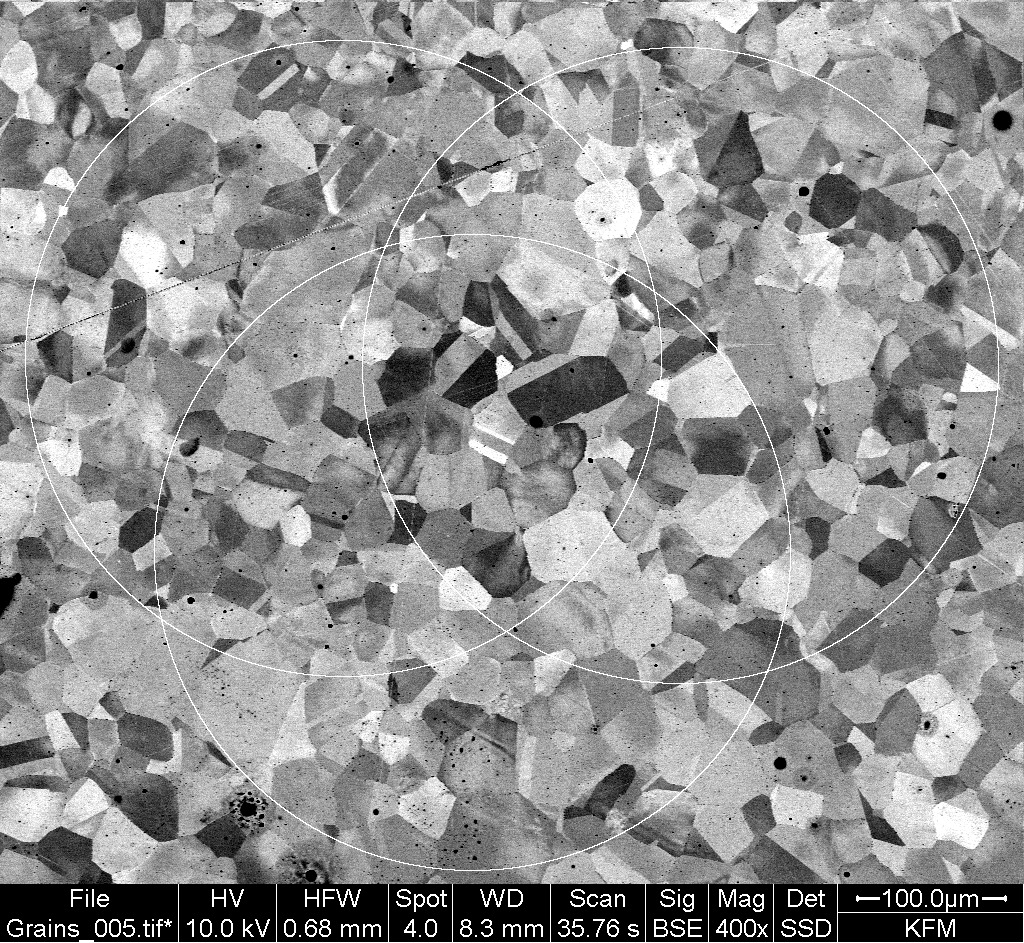
\includegraphics[width=\linewidth]{A18 - SEM/Grains_005_circ.jpg}
        \label{fig:img1}
    \end{minipage}
    \hfill
    \begin{minipage}[b]{0.48\linewidth}
        \centering
        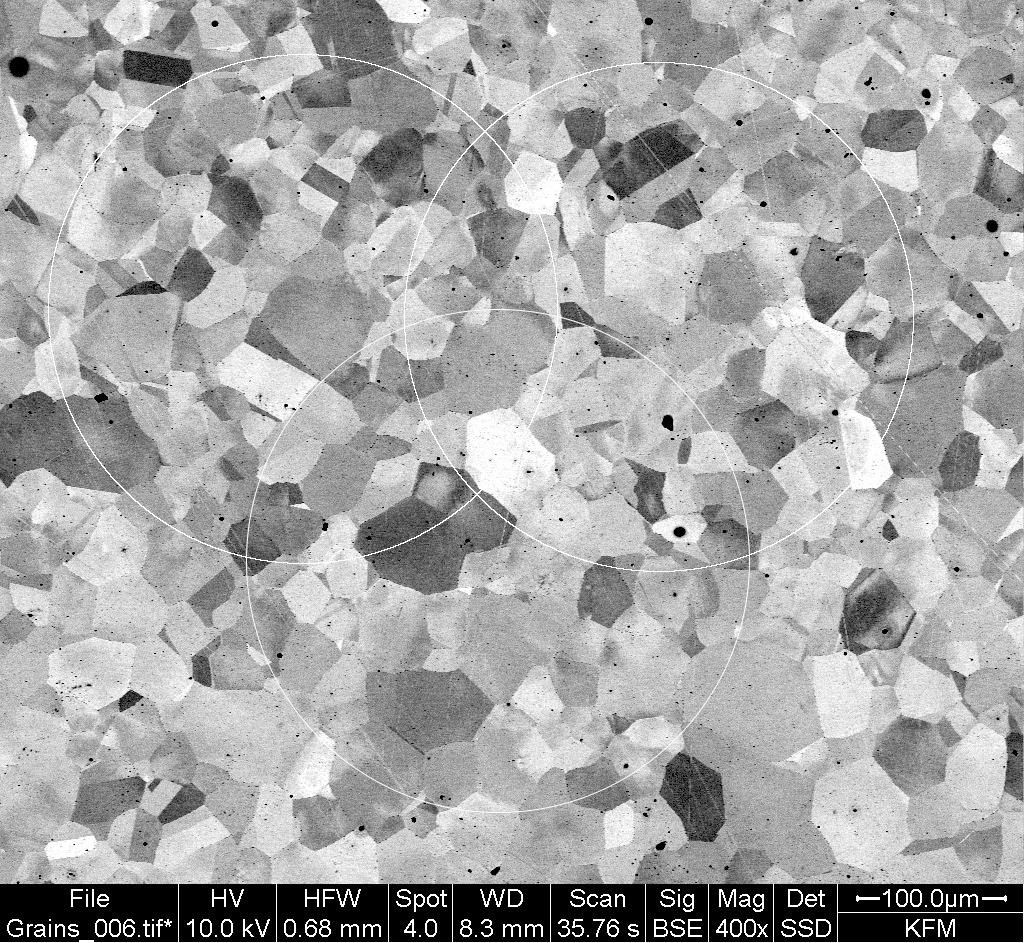
\includegraphics[width=\linewidth]{A18 - SEM/Grains_006_circ.jpg}
        \label{fig:img2}
    \end{minipage}
    
    \vspace{0.5em} % mezera mezi řádky

    \begin{minipage}[b]{0.48\linewidth}
        \centering
        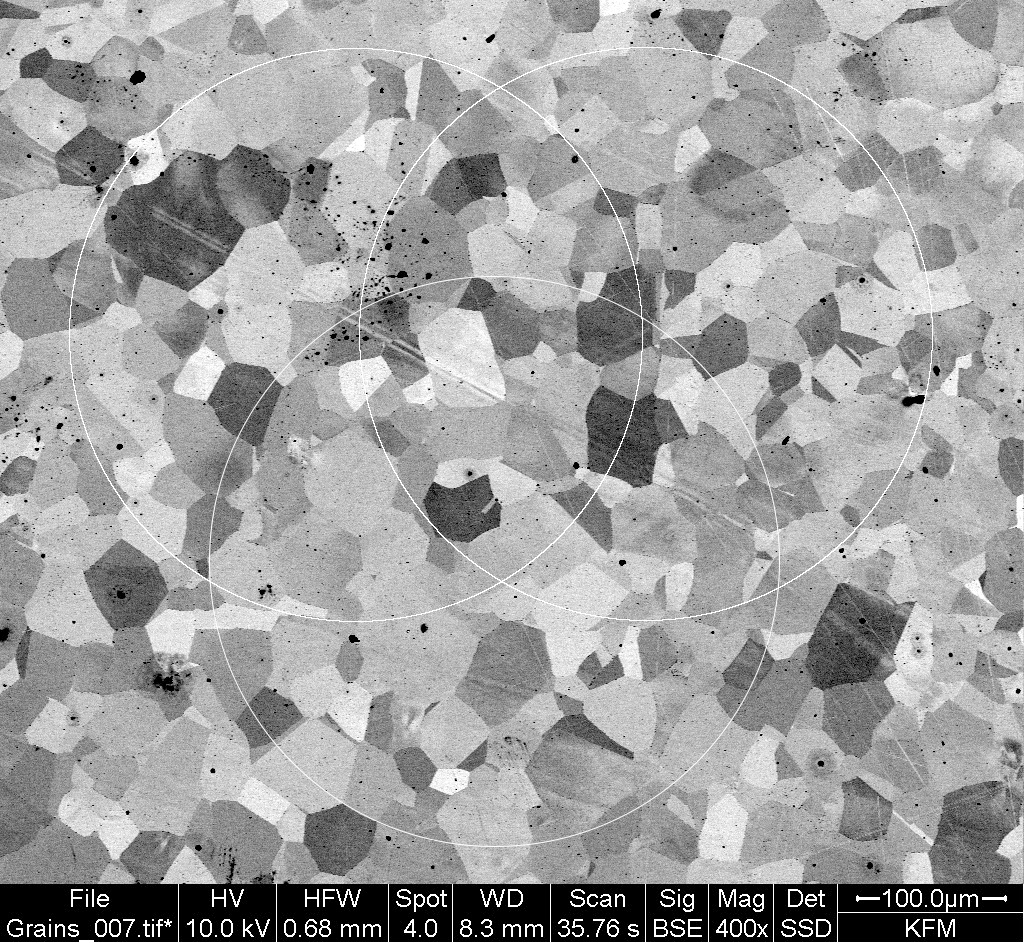
\includegraphics[width=\linewidth]{A18 - SEM/Grains_007_circ.jpg}
        \label{fig:img3}
    \end{minipage}
    \hfill
    \begin{minipage}[b]{0.48\linewidth}
        \centering
        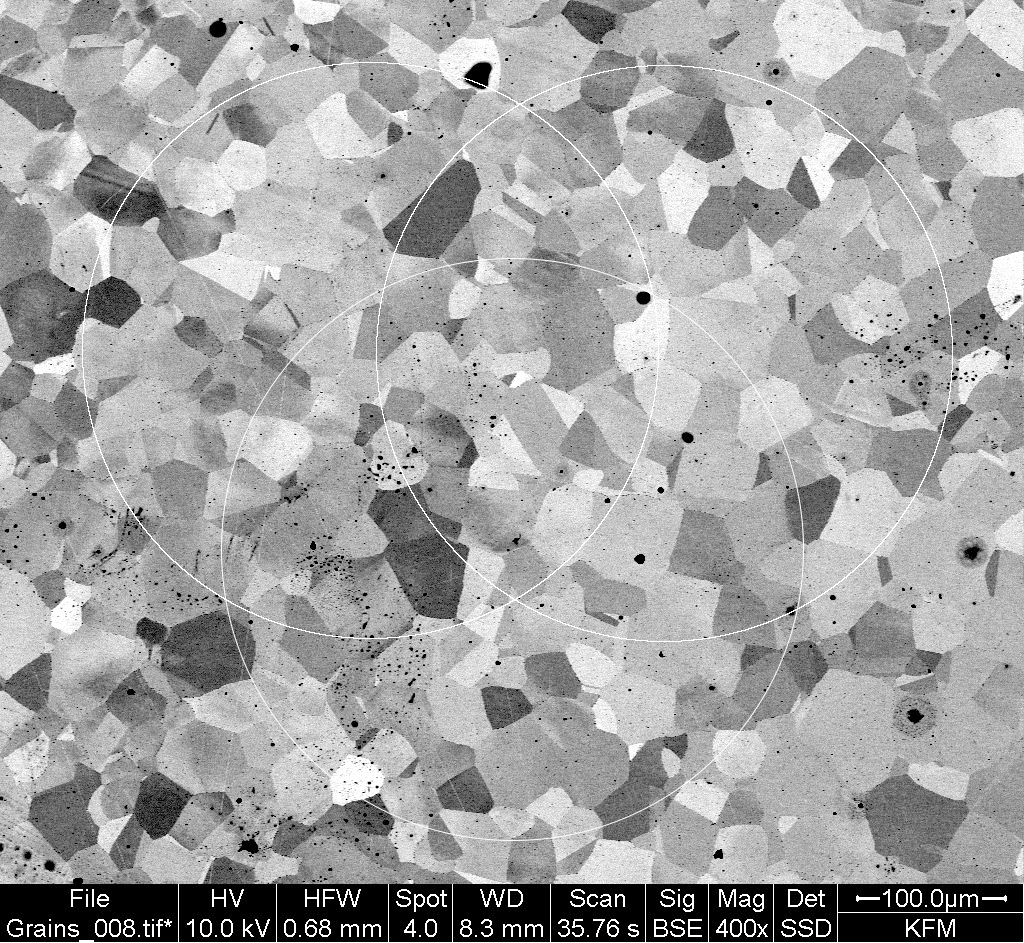
\includegraphics[width=\linewidth]{A18 - SEM/Grains_008_circ.jpg}
        \label{fig:img4}
    \end{minipage}

    \caption{Snímky polykrystalického vzorku }
    \label{fig:lom_rt_all}
\end{figure}

Na každém snímku jsme vyznačili kružnice, přes které budeme zrna sčítat. Zároveň jsme podle metadat obrázků přepočítali průměry těchto kružnic. V tabulce \ref{tab:mereni_zrno} jsou uvedeny výsledky měření kruhovou metodou, kde jsme spočítali střední velikost zrna podle (1). Počet nejistých zrn udává počet zrn, u kterých nebylo možné přesně rozeznat z obrázku, zda se jedná o více zrn, nebo pouze o jedno. Pro další zpracování se jedná o systematickou chybu měření.

\begin{table}[!h]
    \centering
    \renewcommand{\arraystretch}{1.4}
    \setlength{\tabcolsep}{10pt}
    \begin{tabular}{lllll}
        \hline
        \textbf{Vzorek číslo} & \textbf{Poloměr [µm]} & \textbf{Počet proťatých zrn} & \textbf{Počet nejistých zrn} & \textbf{Velikost zrna [µm]} \\
        \hline
        1 & 373{,}3 & 43 & 5 & 40{,}91 \\
        1 & 373{,}3 & 42 & 4 & 41{,}88 \\
        1 & 373{,}3 & 38 & 4 & 46{,}29 \\
        \hline
        2 & 336,0 & 29 & 5 & 54{,}60 \\
        2 & 336,0 & 32 & 5 & 49{,}48 \\
        2 & 336,0 & 32 & 6 & 49{,}48 \\
        \hline
        3 & 378{,}3 & 29 & 7 & 61{,}47 \\
        3 & 378{,}3 & 35 & 5 & 50{,}93 \\
        3 & 378{,}3 & 35 & 4 & 50{,}93 \\
        \hline
        4 & 380{,}3 & 36 & 4 & 49{,}78 \\
        4 & 380{,}3 & 34 & 5 & 52{,}71 \\
        4 & 380{,}3 & 35 & 4 & 51{,}20 \\
        \hline
    \end{tabular}
    \caption{Souhrnná tabulka měření pro čtyři vzorky}
    \label{tab:mereni_zrno}
\end{table}

V tabulce \ref{tab:statistika_zrna} jsou uvedeny výsledky všech měření. Jsou zde zaneseny vypočtené hodnoty průměrné velikosti zrna, standardní odchylka (statistická chyba), systematická chyba a dopočtena celková chyba jako součet kvadrátů předchozích chyb pod odmocninou podle (2).

\begin{table}[!h]
    \centering
    \renewcommand{\arraystretch}{1.3}
    \setlength{\tabcolsep}{8pt}
    \begin{tabular}{llll}
        \hline
        \textbf{Průměr [µm]} & \textbf{Std. odchylka [µm]} & \textbf{Syst. chyba [µm]} & \textbf{Celk. chyba [µm]} \\
        \hline
        49{,}97 & 5{,}44 & 7{,}10 & 8{,}94 \\
        \hline
    \end{tabular}
    \caption{Statistické vyhodnocení velikosti zrna.}
    \label{tab:statistika_zrna}
\end{table}

\subsection{Frakční objem fáze}

Zjišťovali jsme chemické složení pájky, tedy materiálu složeného z cínu a olova. Tyto prvky mají rozdílná atomová čísla, a tedy rozdílný počet elektronů v atomovém obalu. Proto intenzita zpětně odražených elektronů roste s rostoucím atomovým číslem. Olovo má vyšší atomové číslo než cín. Proto pozorujeme olovo jako světlejší místa na snímku v mikroskopu. Na obrázku \ref{fig:sn_pb_combined} jsou zobrazeny dva snímky pro měření chemického složení materiálu. 

\begin{figure}[!h]
    \centering
    \begin{minipage}[b]{0.48\linewidth}
        \centering
        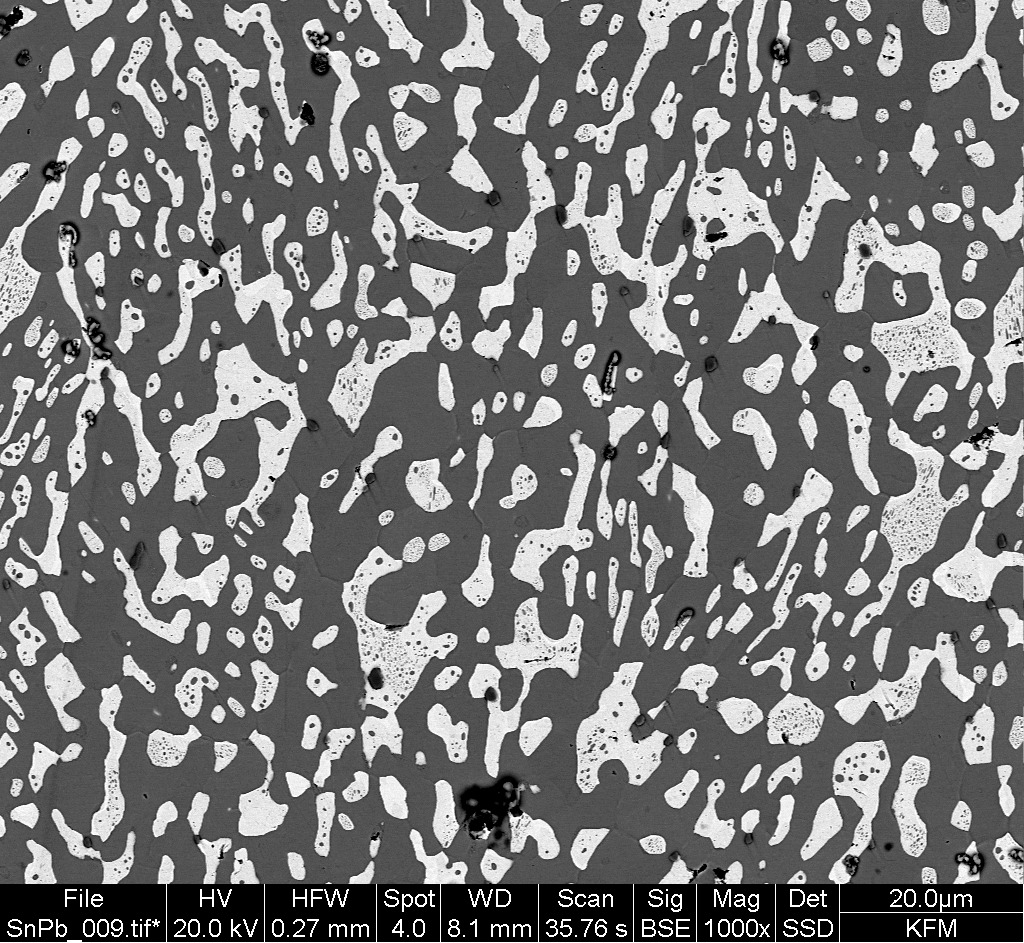
\includegraphics[width=\linewidth]{A18 - SEM/SnPb_009.jpg}
    \end{minipage}
    \hfill
    \begin{minipage}[b]{0.48\linewidth}
        \centering
        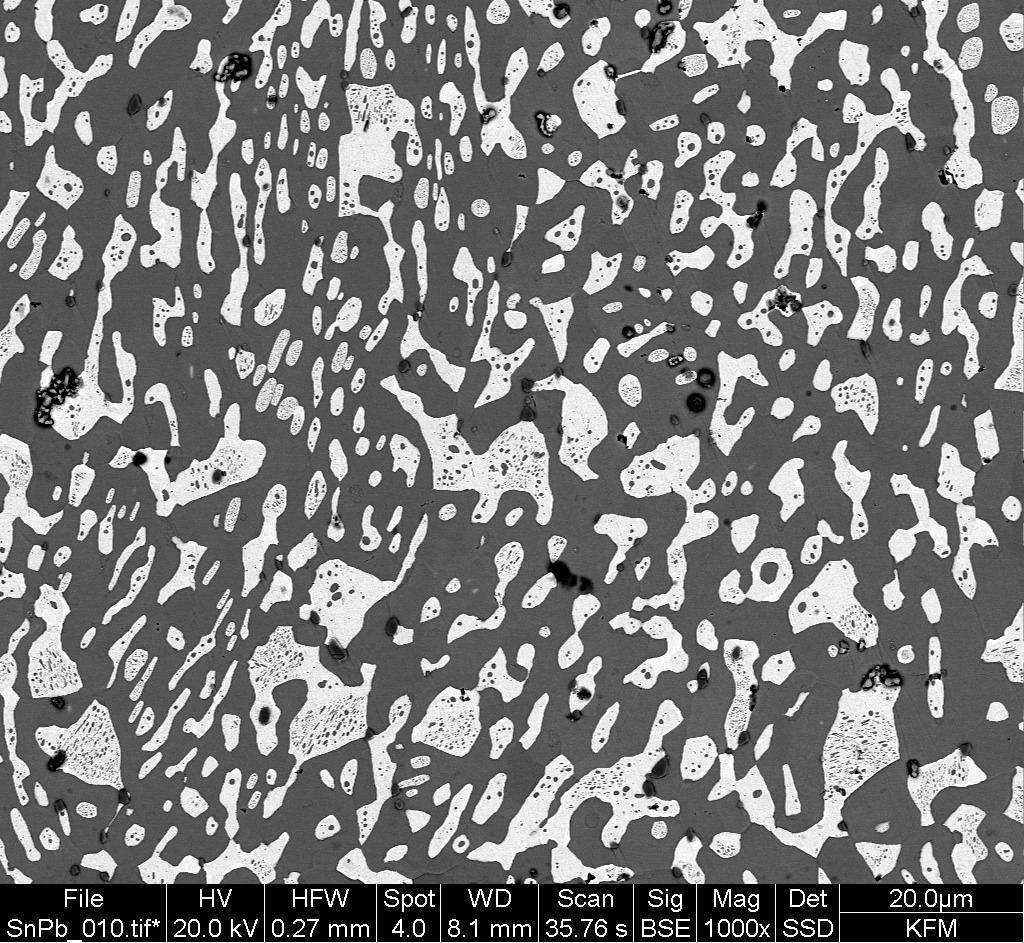
\includegraphics[width=\linewidth]{A18 - SEM/SnPb_010.jpg} % uprav dle potřeby
    \end{minipage}
    \caption{Snímky dvou měření pro určení frakčního objemu dané fáze}
    \label{fig:sn_pb_combined}
\end{figure}

Pomocí programu na zpracování obrazu jsme snímky binarizovali a pomocí histogramu určili procentuální zastoupení jednotlivých odstínů šedi - prvků. Navíc na snímcích pozorujeme černé obrazce, jedná se o nečistoty. Předpokládáme, že poměr zastoupení obou prvků uvnitř nečistot je stejný jako v okolí, proto jsme součet procentuálního zastoupení olova a cínu mohli normalizovat na 100 \%. Nejistotu tohoto měření jsme odhadli změnou oblasti v histogramu, během které jsme nepozorovali viditelný rozdíl ve výběru barevné škály. V tabulce \ref{tab:sn_pb_slozeni} jsou tyto výsledky zobrazeny.

\begin{table}[!h]
    \centering
    \renewcommand{\arraystretch}{1.4}
    \setlength{\tabcolsep}{10pt}
    \begin{tabular}{lll}
        \hline
        \textbf{Prvek} & \textbf{Procentuální zastoupení [\%]} & \textbf{Nejistota [\%]} \\
        \hline
        \multicolumn{3}{l}{\textbf{Měření 1}} \\
        Pb & 35 & 2 \\
        Sn & 65 & 5 \\
        \hline
        \multicolumn{3}{l}{\textbf{Měření 2}} \\
        Pb & 34 & 2 \\
        Sn & 66 & 5 \\
        \hline
    \end{tabular}
    \caption{Složení obou měření – procentuální zastoupení prvků a jejich nejistota}
    \label{tab:sn_pb_slozeni}
\end{table}
    
% ----------------------------------------------------------------------
%  Diskuse výsledků
% ----------------------------------------------------------------------			
\section{Diskuse výsledků}
Na obrázku \ref{fig:lom_rt_combined} pozorujeme také příčný lom. Jedná se o lom kolmý na rovinu zkoumaného lomu. Tato linie je způsobena geometrií jednotlivých zrn, proto může docházet k takovýmto prasklinám. Potvrzuje to křehkost materiálu.

Po zahřátí vzorku v prvním úkolu již nepozorujeme odlišitelná zrna jako ta, která byla patrná před zahřátím. To je v souladu s teoretickým předpokladem, kdy po překročení 600 °C dochází ke zvýšení tažnosti tohoto materiálu podle \cite{bib:studijni-text}.

Zvětšení uvedené v legendě pod obrázkem již při přeškálování obrázku postrádá smysl, jak jsme popsali výše. Vhodné by bylo zanést do obrázku úsečku s její délkou. Bohužel jsme během měření toto zvětšení neurčili, nemůžeme jej nyní uvést.

Celková nejistota měření střední velikosti zrn nám vyšla přibližně 18 \%. Pro vyšší přesnost však narážíme na limity této metody. Průměrná statistická chyba nám vyšla přibližně 14 \% a i s vyšším počtem opakování měření nelze tento typ nejistoty snížit. 

Při měření frakčního objemu dané fáze v materiálu nám obě měření vyšly téměř shodně. Společně s celkovou chybou v řádech jednotek procent můžeme říct, že se jedná o poměrně přesné měření. Navíc při porovnání s \cite{bib:pajka} se výsledné hodnoty shodují s pájkami užívanými v praxi.

% ----------------------------------------------------------------------
%  Závěr
% ----------------------------------------------------------------------
\section{Závěr}

Pomocí skenovací elektronové mikroskopie jsme nejprve studovali lomové plochy materiálu $Fe_3Al$ tažené při různých teplotách a snímky jsme vyhodnotili a vysvětlili.

Dále jsme pomocí kruhové metody určili střední velikost zrn $d$ polykrystalického materiálu jako

\begin{equation}
    \nonumber
    d = (50 \pm 9) \; \mu m
\end{equation}

Nakonec jsme pomocí zpětně odražených elektronů určili chemické složení (poměr olova a cínu) v pájce ve dvou měřeních. V prvním z měření jsme změřili, že olovo je zastoupeno ze 35 \% a cín z 65 \%. V druhém měření pak olovo 34 \% a cín 65 \%.